\documentclass[10pt,letterpaper]{article}
\usepackage{geometry}
\geometry{margin=1in}
\usepackage{graphicx}

\setlength{\parindent}{0pt}
\setlength{\parskip}{0.5em}

\usepackage{enumitem}
\setlist{nolistsep}

\usepackage{titlesec}
\titlespacing*{\section}{0pt}{0\baselineskip}{0\baselineskip}
\titlespacing*{\subsection}{0pt}{0\baselineskip}{0\baselineskip}
\titlespacing*{\subsubsection}{0pt}{0\baselineskip}{0\baselineskip}

\usepackage{enumitem}
\setlist{nosep}

\usepackage[hidelinks]{hyperref}

\title{Lab 2 - Linguistics Data, STAT 215A, Fall 2026\vspace{-2em}}

\begin{document}
\maketitle

\section{Introduction}\label{introduction}

Ask two people from the same city how they address a group of strangers, or
what they call a fizzy drink, and there is a good chance they will not answer
alike, but ask the same question of two people three hundred miles apart and
the odds of agreement drop sharply. American English varies systematically
with geography, and Bert Vaux's Dialect Survey was built to measure exactly
that: 47,471 respondents answering the same lexical questions, geolocated by
the ZIP codes they reported.

Measuring the geography is the easy part; interpreting it is not. Any single
word's distribution is a tangle of local pockets, migration, and contact, so
dialectometry aggregates many variables at once. Nerbonne and Kretzschmar's
2003 introduction frames dialectometry as the computational counterpart of
dialectology, the measurement of variation whose distribution is primarily
geographic, and their 2006 follow-up argues that the payoff comes from
explaining aggregate patterns rather than individual words. That is the logic
here: two words alone, then four, then all 67, and finally a clustering of
every respondent, with each step asking whether the structure that emerges is
geography showing through or an artifact of the encoding.

\section{The Data}\label{data}

Bert Vaux's Dialect Survey put roughly one hundred questions to 47,471
respondents across the United States, and this analysis uses three files from
it. \texttt{lingData.txt} is the respondent-level data: one row per person, 73
columns wide, holding an anonymous \texttt{ID}, the city, state and ZIP code
each respondent typed in, their answers to the 67 lexical questions in the
range Q050--Q121, and a latitude and longitude derived from their ZIP code.
Almost everyone answered almost everything, so the interesting question is what
people \emph{say} rather than whether they answered.

The answers arrive as integers rather than words. A 0 means the question was
not answered; any other number indexes the survey's published answer letters,
so a 1 means the respondent picked option (a). \texttt{question\_data.RData}
supplies the question wording and the answer letters for every item, so Q50 can
be read as ``what word do you use to address a group of two or more people?''
and its code 4 as \emph{you guys}. This analysis loads that file with
\texttt{pyreadr} to turn codes into labels wherever answers are named in text
or figures.

The third file, \texttt{lingLocation.txt}, holds no new respondents. It is the
same answers re-encoded geographically: each person's answers become a binary
indicator vector, and everyone sharing a one-degree square of latitude and
longitude is \emph{summed} into one row for that cell. A cell read 50 for
``soda'' therefore means 50 people in that square said soda, not that 50 is a
proportion. Only Section~\ref{clustering} uses these cells, and
Section~\ref{separators} shows why that turns out to be the fragile part of
the analysis; everything else works at the respondent level. Map overlays
follow the pattern in \texttt{code/demo.ipynb}.

\subsection{Data Cleaning}\label{data-cleaning}

The data are messier than they look, and the mess is worth naming because
several cleaning choices are judgment calls that affect later results.

\textbf{No-response codes.} 3.17\% of all answer cells are 0, with per-question
response rates from 91.8\% (Q092, lane-changing) to 97.3\% (Q050, Q052, Q054,
Q056, Q063). A 0 conflates two different situations: respondents who skipped
the question, and respondents who genuinely have no word for the concept.
Q064 offers an explicit ``I have no word for this'' (code 10, 0.9\% of
respondents), so a 0 is not the same as a shrug. I keep 0s as zeros through the
binary encoding rather than dropping rows, since dropping would discard
geography: respondents who skipped Q50 still answered Q105 and still have a
location.

\textbf{State codes.} \texttt{STATE} has 92 distinct values, of which 159 rows
are not US states: \texttt{XX} placeholders (84 rows), Canadian provinces
(\texttt{ON}, \texttt{NB}, \texttt{BC}, \texttt{QC}, \texttt{NS}, \texttt{AB}),
\texttt{UK}/\texttt{NZ}/\texttt{IE}/\texttt{PR}, and outright typos
(\texttt{00}, \texttt{94}, \texttt{C)}, \texttt{!L}). These rows are flagged
via \texttt{state\_valid} rather than dropped. At 159 of 47,471 they cannot
move any regional statistic, and dropping them silently would hide a real
data-entry problem worth reporting.

\textbf{Geocoding.} 1,020 respondents have no coordinates, leaving 46,245
mappable; 206 more fall outside a continental bounding box because the ZIP
centroids fall in Alaska, Hawaii, or outside the country. Because coordinates
come from ZIP centroids rather than respondent-reported positions, they are
only as precise as the ZIP code area, which is fine for regional patterns and
poor for anything finer. All of this lives in \texttt{code/clean.py}, whose
\texttt{clean\_data} copies its input and returns a new frame with
\texttt{state\_valid} and \texttt{geo\_valid} flags, so each decision above is
recorded once and applied everywhere downstream.

\section{Exploratory Data Analysis}\label{data-exploration}

\subsection{Two questions and their geography}

I focus on Q50 (what word do you use to address a group of two or more
people?) and Q105 (your general term for a sweetened carbonated beverage).
Among the 46,205 respondents who answered Q50, the split is \emph{you guys}
42\%, \emph{you} 24\%, \emph{y'all} 18\%, \emph{you all} 13\%. Among the 46,098
who answered Q105 it is \emph{soda} 48\%, \emph{pop} 28\%, \emph{coke} 14\%.
Restricted instead to respondents giving one of the three standard beverage
words, the Q105 split is 53/31/16 and Q50 is 44/25/18/13. Figure~\ref{fig:maps} shows both mapped,
and the two answer different questions about the country. Grouping the
respondents into four Census-style regions, defined as in Table~\ref{tab:regions}
(the Census South, so Delaware, Maryland and DC are counted as South), shows how
sharply: \emph{coke} reaches 41.4\% in the South and under 10\% everywhere
else, \emph{soda} takes 81.3\% of the Northeast, and \emph{pop} leads the
Midwest at 55.2\%. The West is the interesting case: majority \emph{soda} at
55.1\% but a substantial \emph{pop} minority at 33.8\%, which is why the
country is not cleanly split in two.

\begin{table}[h]
\centering
\begin{tabular}{lrrr}
\hline
Region & \emph{soda} & \emph{pop} & \emph{coke} \\
\hline
Northeast & 81.3 & 13.2 & 5.5 \\
Midwest & 35.6 & 55.2 & 9.2 \\
South & 46.8 & 11.7 & 41.4 \\
West & 55.1 & 33.8 & 11.0 \\
\hline
\end{tabular}
\caption{Q105 answers by region (percent of respondents in that region giving
each answer). Regions follow the Census (South includes DE, MD and DC); 1,020
respondents without usable coordinates and 159 with unusable state codes are
excluded, leaving 46,292. Sample shares: Midwest 34.5\%, Northeast 24.6\%,
South 22.6\%, West 18.3\%.}
\label{tab:regions}
\end{table}

\begin{figure}[h]
\centering
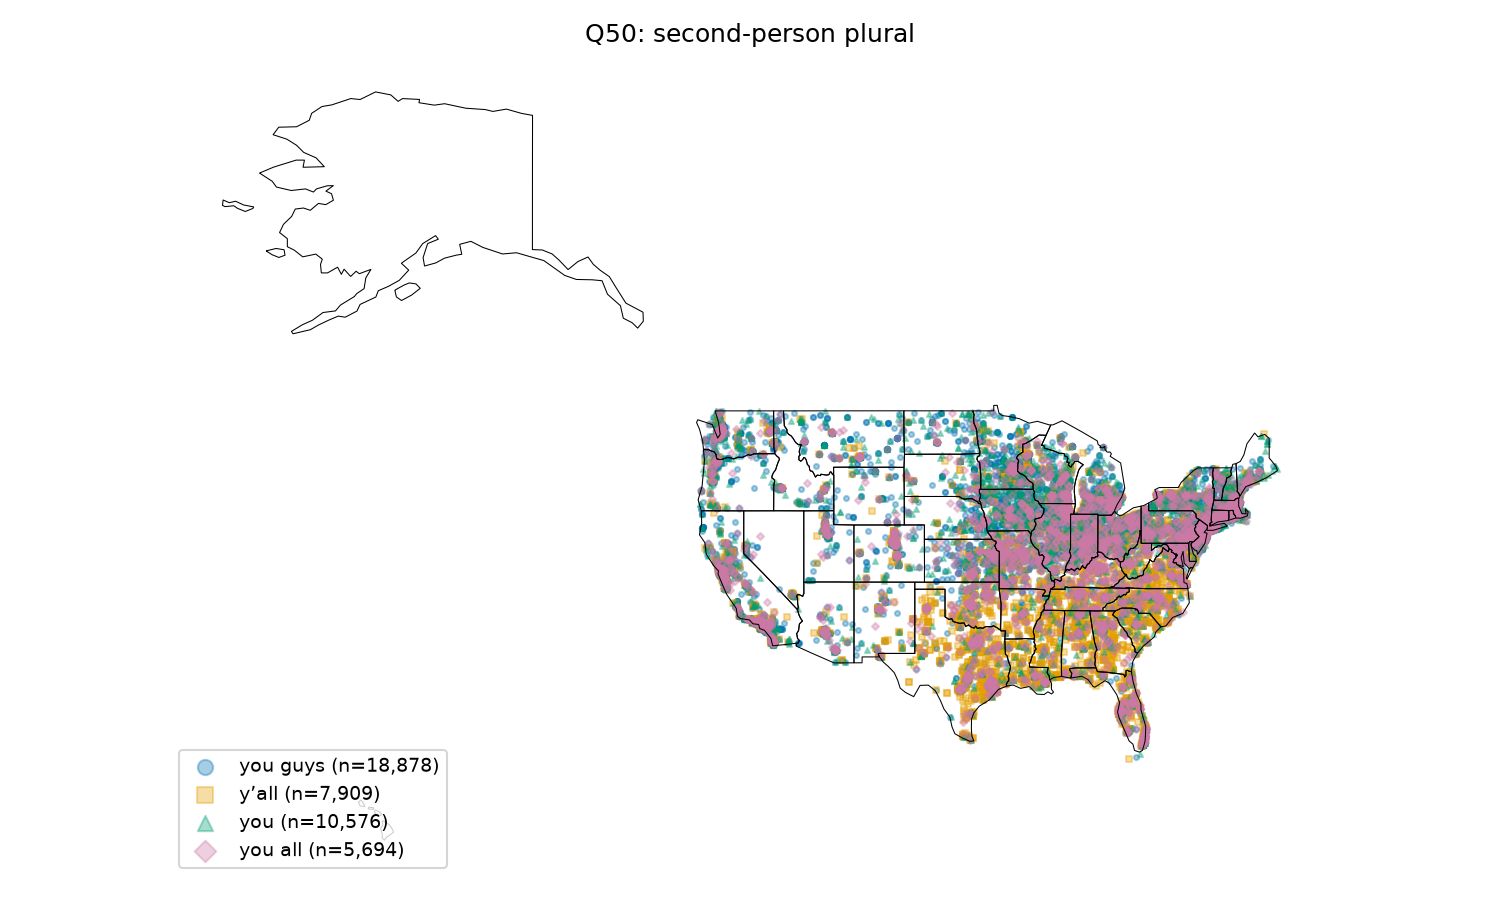
\includegraphics[width=0.49\textwidth]{../figs/q50_map.png}
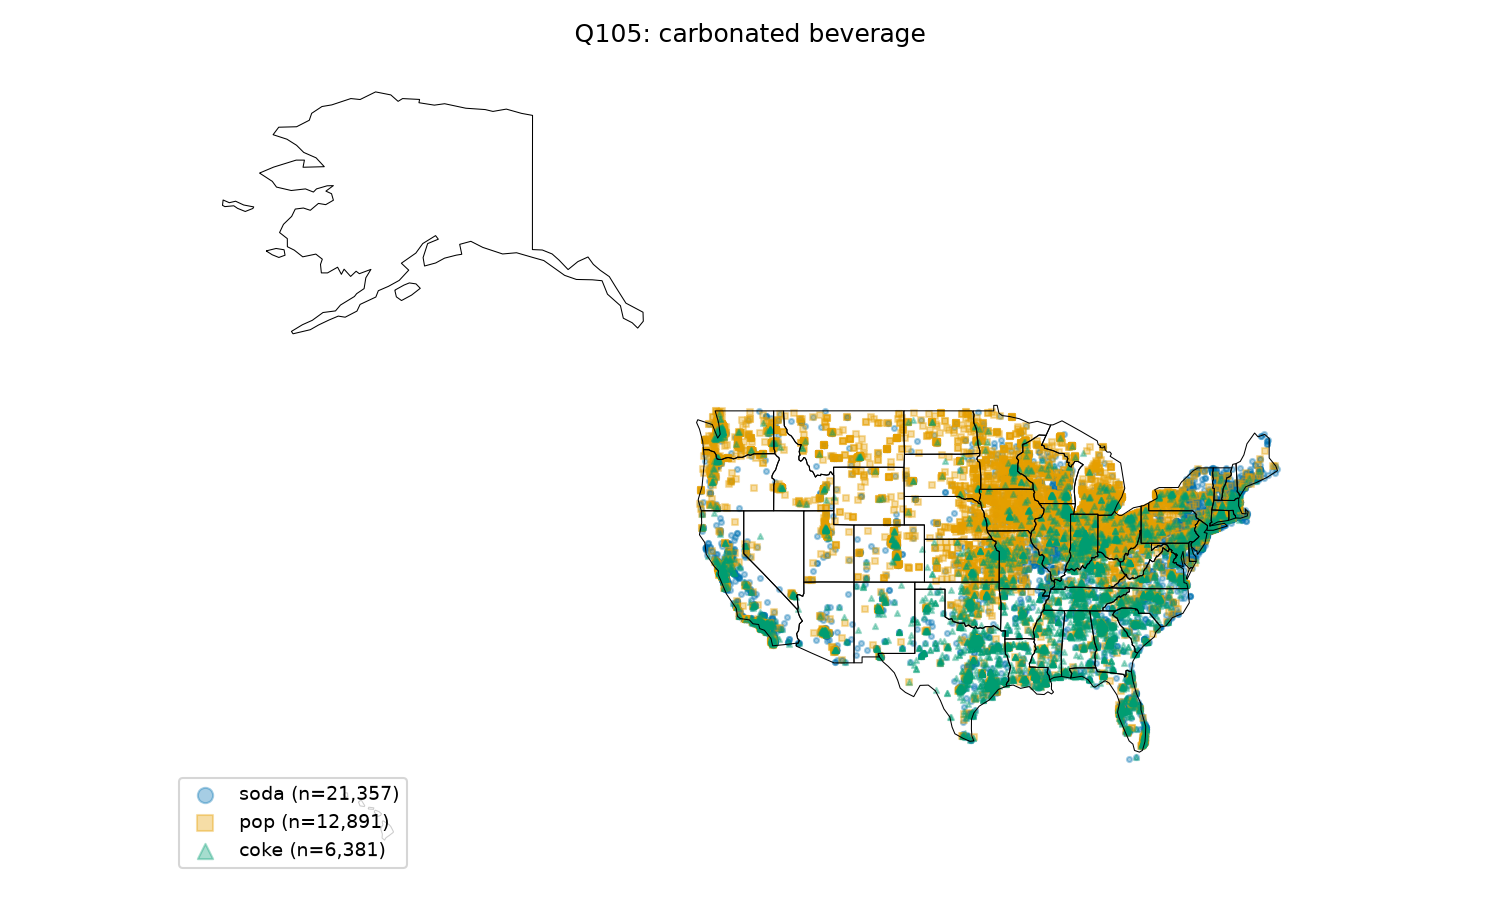
\includegraphics[width=0.49\textwidth]{../figs/q105_map.png}
\caption{Q50 (left) and Q105 (right) answers by respondent location.}
\label{fig:maps}
\end{figure}

The survey's own published percentages, carried in
\texttt{question\_data.RData}, are a useful external check: our subset closely
reproduces them on the standard-answer denominator (Q105 \emph{soda} 53.0\%
reported against 52.9\% here; Q50 \emph{you} 24.8\% against 24.6\%). The
substantive differences are \emph{pop} (25.1\% reported, 31.4\% here) and
\emph{y'all} (14.0\% against 18.3\%), so this PUD subset skews slightly Southern
in exactly the direction of the effects I report.

Q64 and Q103 are geographically precise in a different way. Q64
(\emph{sub} / \emph{hoagie} / \emph{hero} / \emph{grinder}) is the standard
textbook illustration of an enclave rather than a gradient:
\emph{hoagie} is given by 15.7\% of respondents in the Northeast against
3.9\% everywhere else. Q103 is the reverse case: \emph{bubbler} (water fountain
in schools) is given by 33.8\% of respondents in WI/MA/RI against 1.3\%
elsewhere, a genuinely local word with a tiny footprint. Q73
(\emph{sneakers} vs \emph{tennis shoes}) leans Southern too, though only
mildly (56.6\% vs 44.0\% for \emph{tennis shoes}).

\begin{figure}[h]
\centering
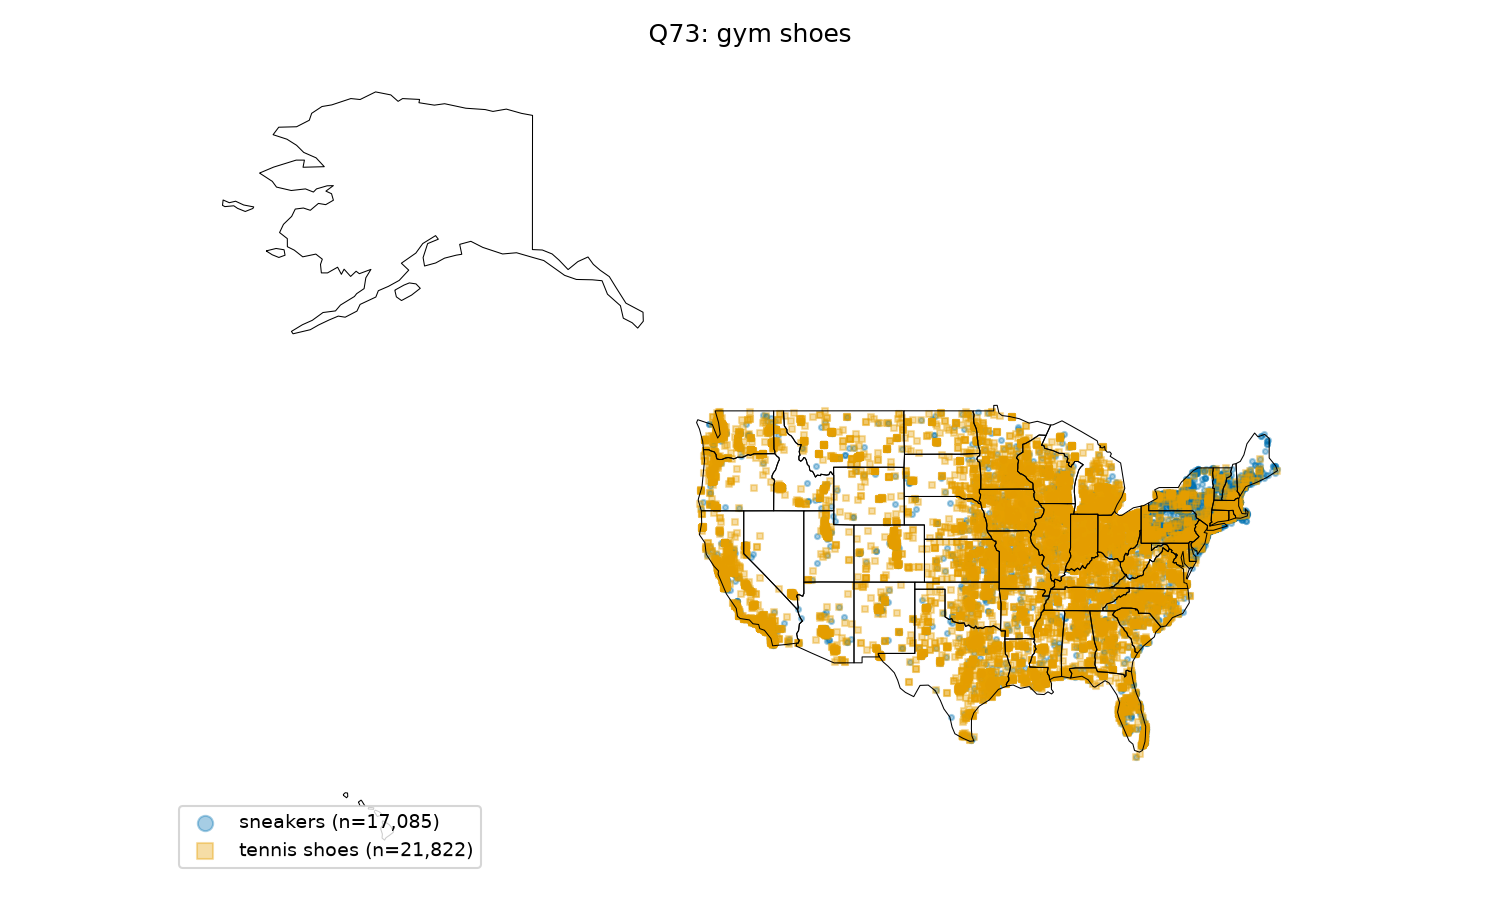
\includegraphics[width=0.49\textwidth]{../figs/q73_map.png}
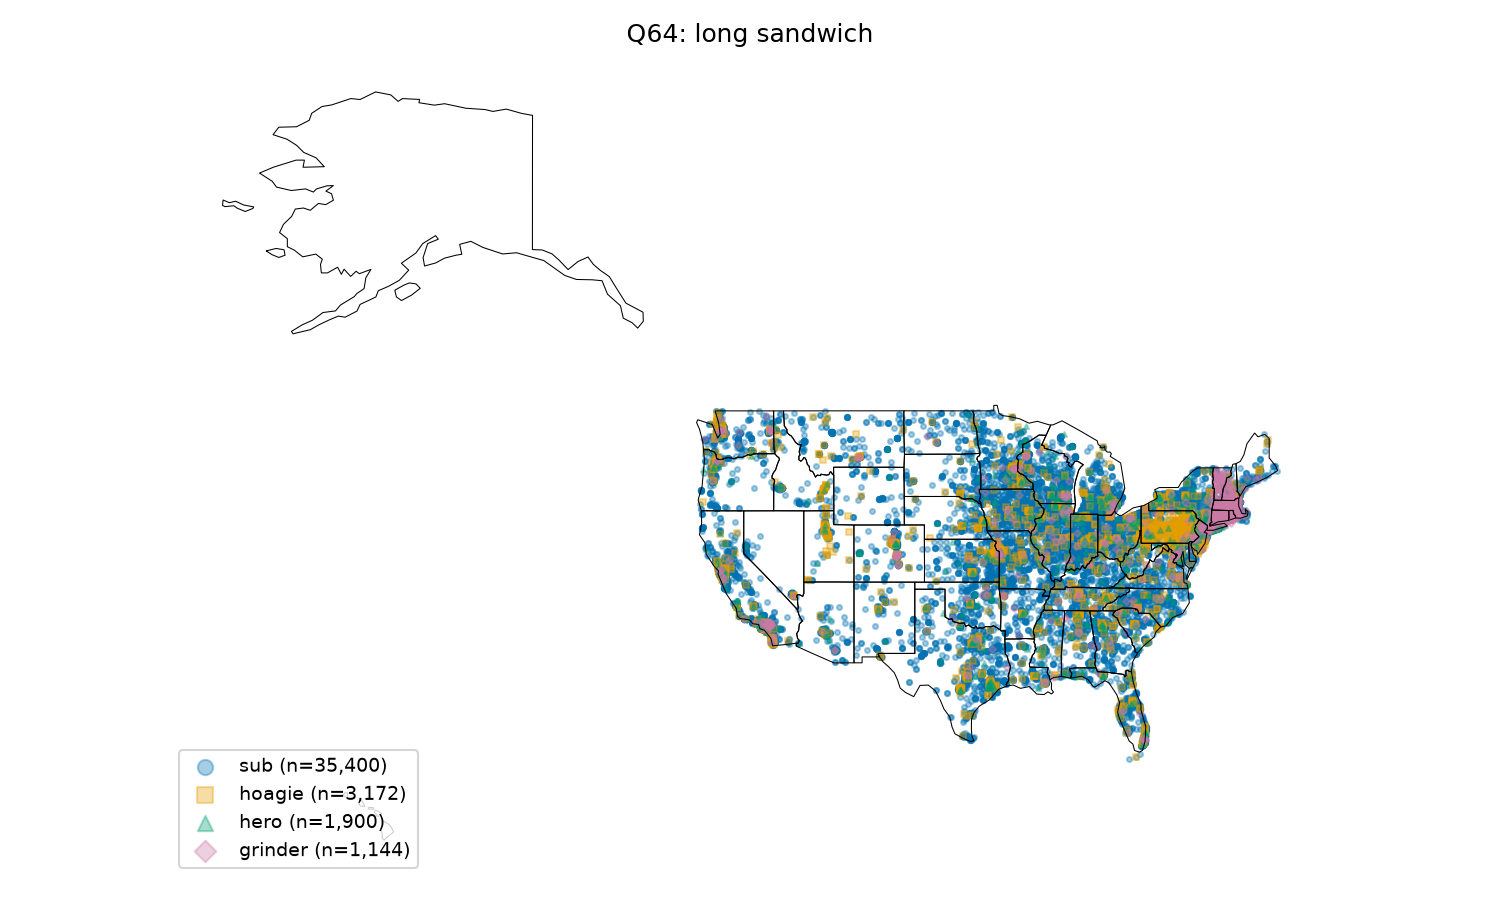
\includegraphics[width=0.49\textwidth]{../figs/q64_map.png}
\caption{Q73 (left): \emph{tennis shoes} skew Southern. Q64 (right): the Philadelphia
\emph{hoagie} pocket.}
\label{fig:maps2}
\end{figure}

The scatter maps overplot tens of thousands of points, so density is hard to
read. Figure~\ref{fig:prob} replaces them with a KNN-smoothed probability
surface (100 nearest neighbours in lon/lat, distance-weighted), which answers
the region-versus-gradient question directly: \emph{coke} never exceeds
P = 0.85 anywhere and holds a majority over only 13\% of the grid, \emph{pop}
covers 27\%, and \emph{soda} 47\%. Three broad surfaces with soft, overlapping
edges is itself evidence for the continuum reading in
Section~\ref{continuum}.

\begin{figure}[h]
\centering
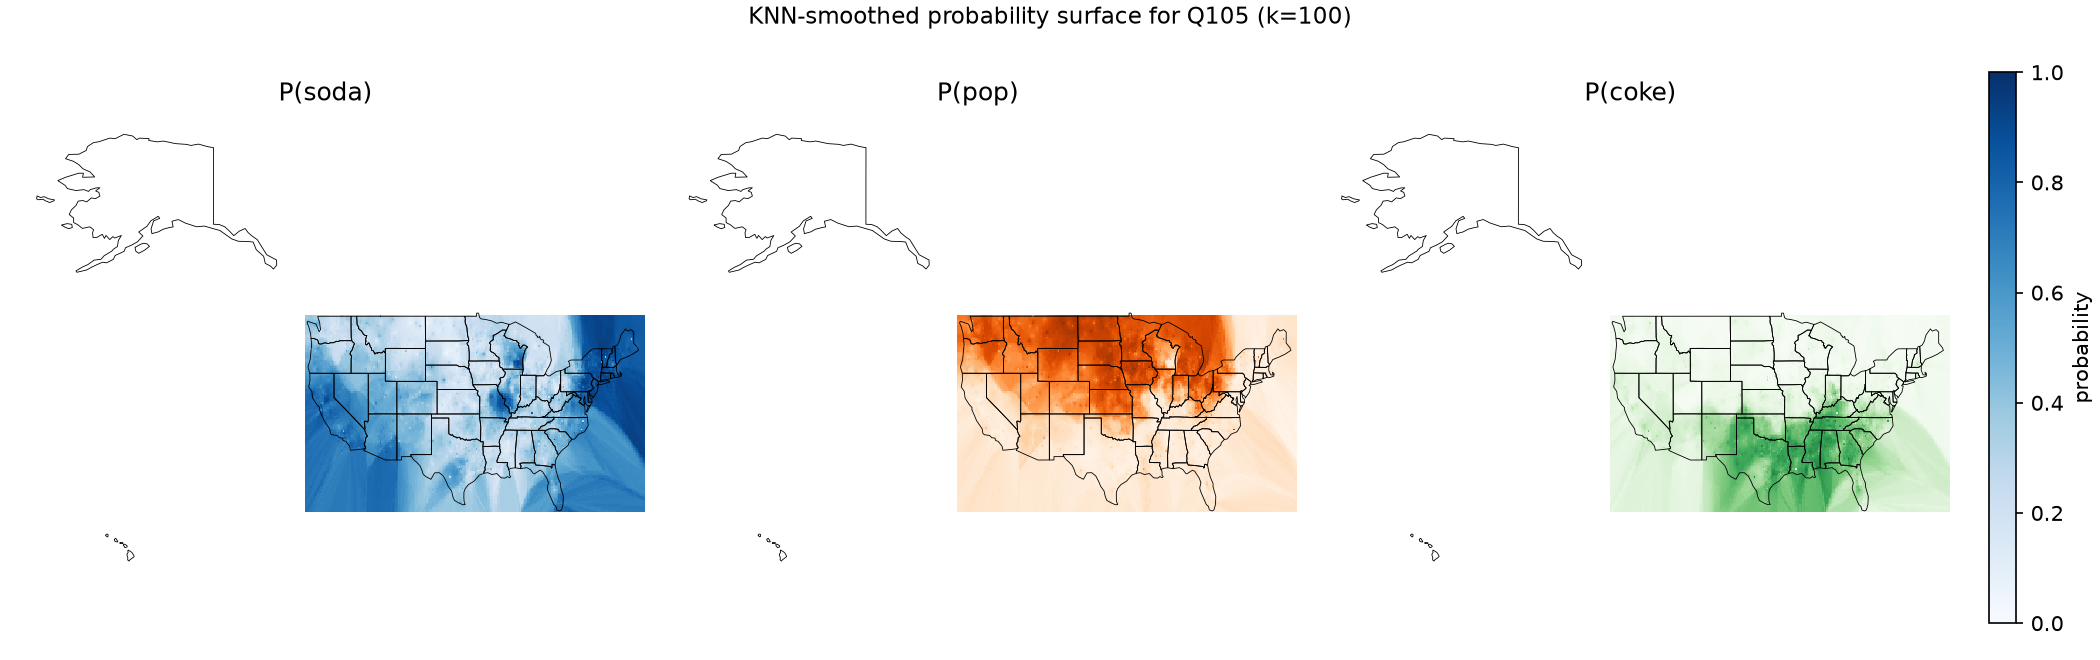
\includegraphics[width=0.80\textwidth]{../figs/q105_probability_map.png}
\caption{KNN-smoothed probability of each Q105 answer across the continental
US. The three surfaces meet in soft transitions rather than sharp borders.}
\label{fig:prob}
\end{figure}

Because static maps hide which words co-occur in the same mouths, I also built
an interactive version (Figure~\ref{fig:plotly}); hovering any point reports
that respondent's Q50 answer alongside their map color, which makes the
coke/\emph{y'all} overlap in the Deep South directly visible.

\begin{figure}[h]
\centering
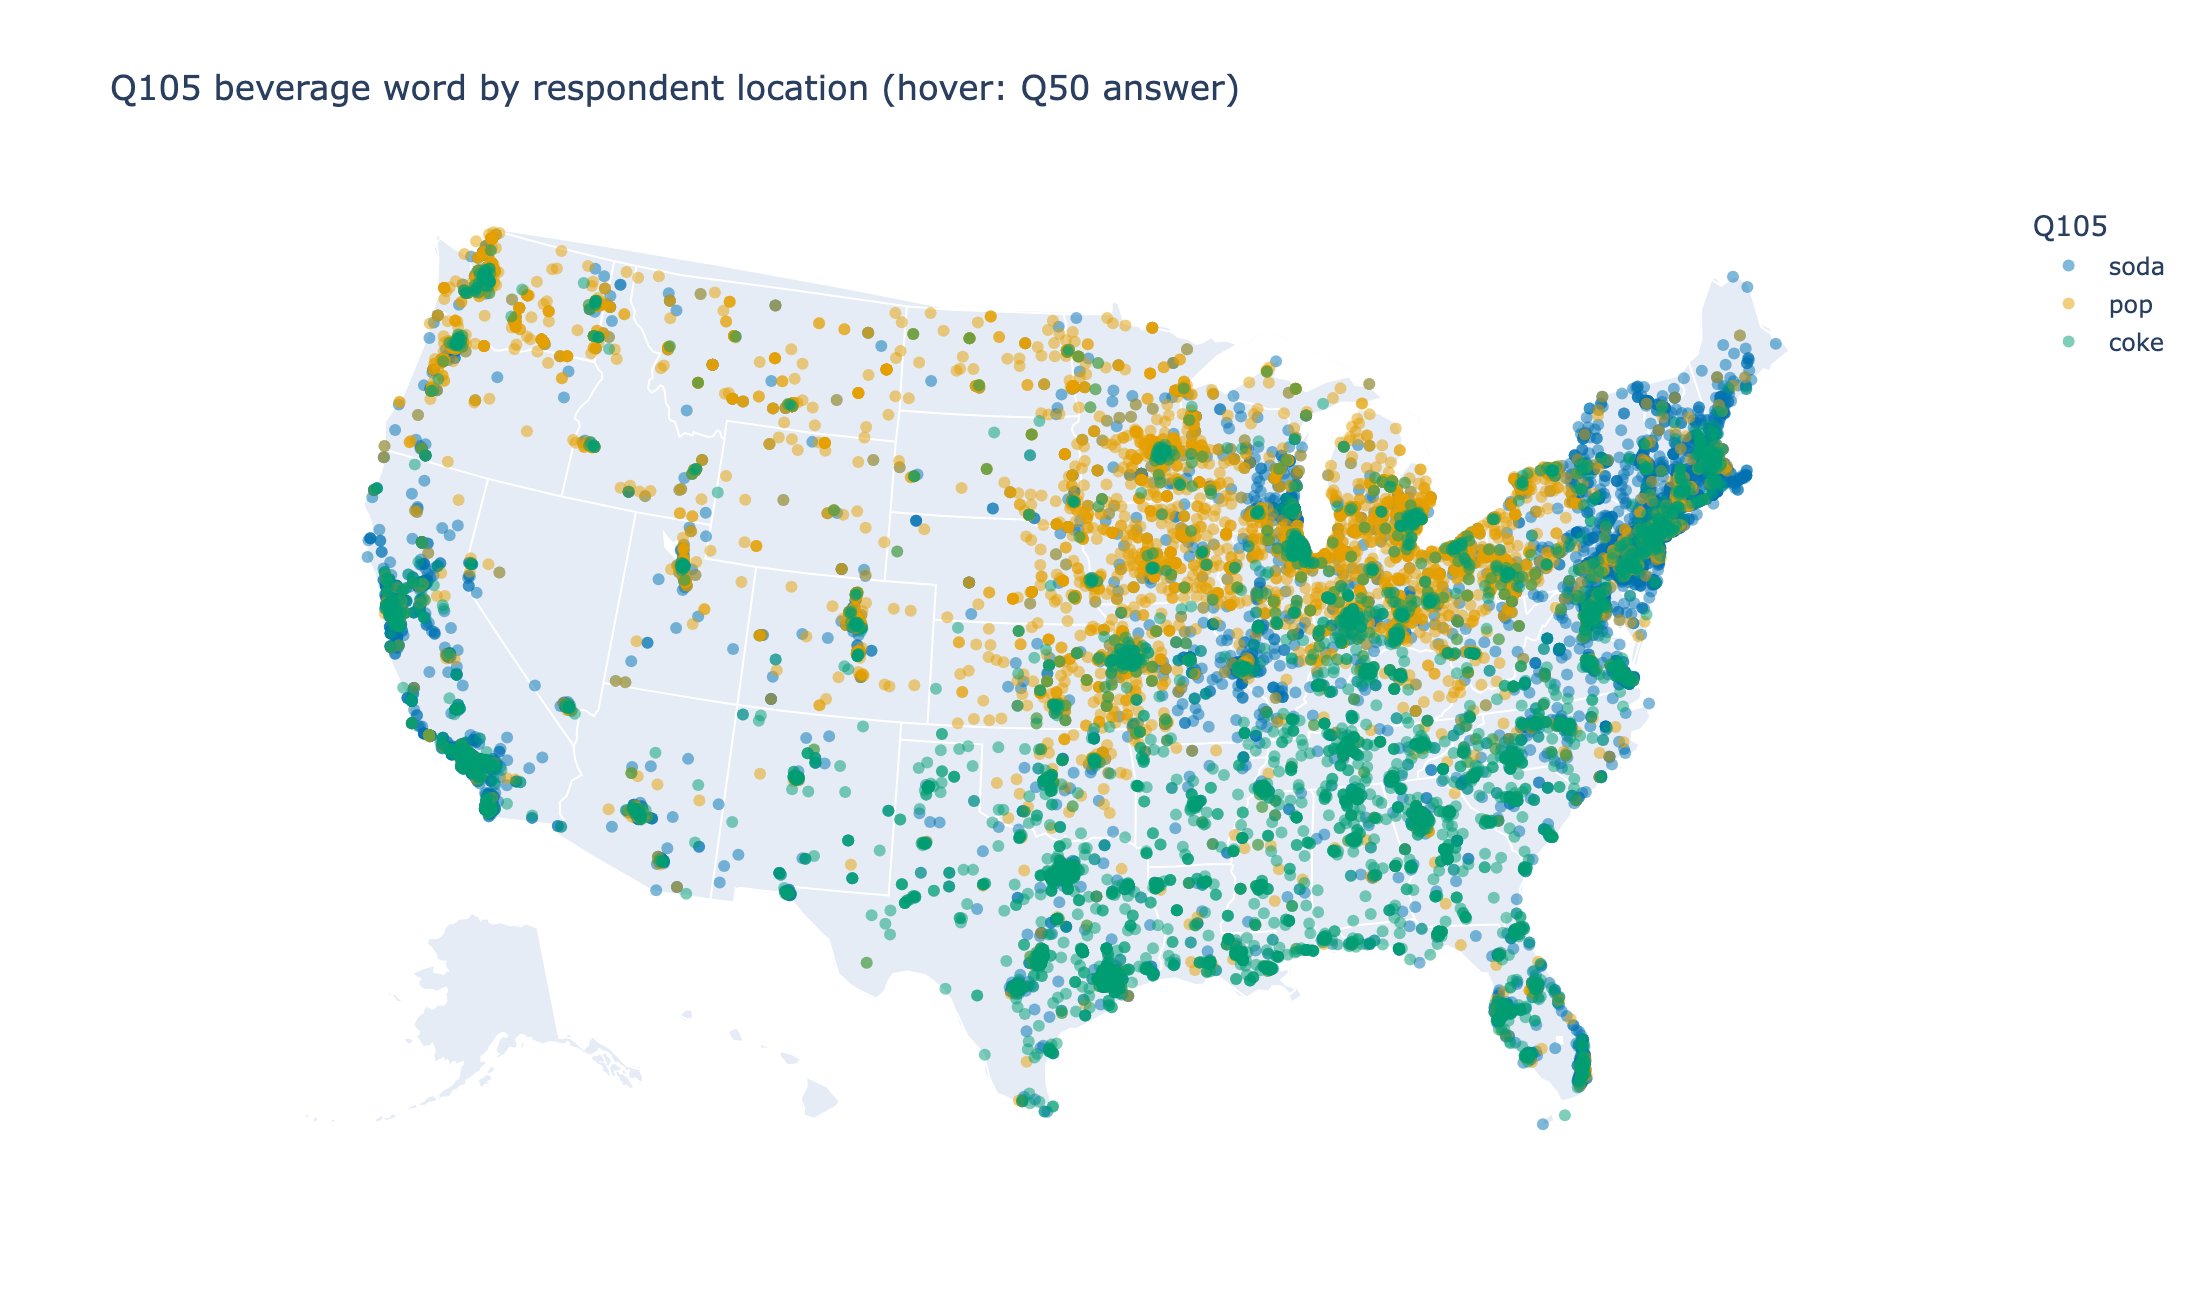
\includegraphics[width=0.85\textwidth]{../figs/plotly_q105_map.png}
\caption{Q105 by location, exported from the interactive Plotly version
(\texttt{figs/interactive\_q105.html}, bundled for offline hover/zoom). The
interactive version plots the 24,579 respondents who gave \emph{soda},
\emph{pop}, or \emph{coke} and answered Q50 with \emph{you guys} or
\emph{y'all}.}
\label{fig:plotly}
\end{figure}

\subsection{Does one answer help predict the other?}

Screening all 2,211 question pairs first (Section~\ref{separators}) shows
that Q50$\times$Q105 is well above the median pair association but is not the
most strongly associated pair in the survey: kinship terms (Q070$\times$Q071,
V = 0.414) and the \emph{anymore} sentences (Q054$\times$Q055, V = 0.417) are
stronger. Those pairs are near-deterministic within families, whereas Q50 and
Q105 were picked for geographic reach rather than raw association, which is the
trade I wanted.

The two questions are not independent. Among respondents answering both,
P(\emph{y'all} $\mid$ \emph{coke}) = 58.3\%, against 6.0\% given \emph{pop}
and 12.2\% given \emph{soda}, roughly a tenfold lift. Cram\'er's V over the
full four-by-three table is 0.276 (n = 42,320). The association is
asymmetric: knowing someone says \emph{coke} says a great deal about their
pronoun, whereas knowing \emph{y'all} says much less about their drink, because
\emph{you guys} is the majority answer nearly everywhere and so carries little
information about the beverage word.

Table~\ref{tab:joint} shows the joint distribution behind these numbers. The
\emph{coke} column holds 3,684 \emph{y'all} respondents while the \emph{pop}
column holds only 750, a nearly fivefold difference that is almost entirely a
\emph{y'all}-vs-\emph{you guys} split: \emph{you guys} is 57.3\% of the
\emph{pop} column but only 23.1\% of the \emph{coke} column.

\begin{table}[h]
\centering
\begin{tabular}{lrrrr}
\hline
 & \emph{soda} & \emph{pop} & \emph{coke} & other \\
\hline
\emph{you all} & 2,775 & 1,647 & 673 & 477 \\
\emph{you guys} & 9,577 & 7,140 & 1,460 & 543 \\
\emph{you} & 6,076 & 2,928 & 500 & 873 \\
\emph{y'all} & 2,560 & 750 & 3,684 & 657 \\
\hline
\end{tabular}
\caption{Q50 rows by Q105 columns (respondents answering both, n = 42,320).
Cram\'er's V = 0.276.}
\label{tab:joint}
\end{table}

Turning that into an actual prediction makes the asymmetry precise. Among the
respondents who gave one of the three beverage words, 15.7\% say \emph{coke}.
Predicting that binary outcome from Q50 alone with a one-hot logistic model
reaches 85.2\% accuracy under five-fold cross-validation, 5.4 times the base
rate's error rate, and adding Q73 raises it to 87.6\%. A single
lexical question therefore carries substantial information about an unrelated
one, which is precisely the aggregation argument Nerbonne and Kretzschmar
make: individual variables are noisy, but their joint geography is not.

\subsection{Beyond two questions}

Extending to four questions shows one dominant axis and several local ones.
The pairwise associations rank Q50$\times$Q105 first (V = 0.276), then
Q105$\times$Q73 (0.187), Q105$\times$Q64 (0.164), Q73$\times$Q64 (0.145), with
both Q50 cross-questions weakest (0.077 and 0.082). The pattern is what
dialectometry predicts: a broad north--south axis that many words share, plus
sharp local enclaves (\emph{hoagie}, \emph{bubbler}) that participate in
almost no large-scale structure. Answer codes used throughout are listed in
Table~\ref{tab:codes}.

\begin{table}[h]
\centering
\begin{tabular}{lll}
\hline
Question & Codes used & Answers \\
\hline
Q50 & 1, 4, 7, 9 & \emph{you all}, \emph{you guys}, \emph{you}, \emph{y'all} \\
Q105 & 1, 2, 3 & \emph{soda}, \emph{pop}, \emph{coke} \\
Q73 & 1, 6 & \emph{sneakers}, \emph{tennis shoes} \\
Q64 & 1, 3, 4, 2 & \emph{sub}, \emph{hoagie}, \emph{hero}, \emph{grinder} \\
Q103 & 1, 4 & \emph{bubbler}, \emph{water fountain} \\
\hline
\end{tabular}
\caption{Question codes used in this report, as returned by
\texttt{question\_data.RData}.}
\label{tab:codes}
\end{table}

\section{Dimension Reduction}\label{dimension-reduction}

\subsection{Encoding}

Encoding every (question, answer) pair as a binary indicator turns 67
categorical questions into a (47,471 $\times$ 468) binary matrix at 13.9\%
density, the $p = 468$ given in the instructions. Answers like Q065's
``I use lightning bug and firefly interchangeably'' become their own column
alongside the two individual answers, and a 0 (no response) contributes zeros
across that question's whole block.

\subsection{Centering and scaling, and why not PCA on the raw categories}

Two choices matter here, and the instructions ask for both to be defended.
\emph{Centering} is handled internally by scikit-learn's PCA, so uncentered and
centered fits are identical; I report both to make that explicit. On the
resulting components, PC1 explains 4.03\% of variance and PC2 3.46\%, with
10 components covering 23.15\%): a flat spectrum, which for 468 sparse
dimensions is expected and itself informative: there is no small set of
dominant directions, because each component is a diffuse regional mixture.

\emph{Scaling} is where I deviate from the default. Standardizing every column
to unit variance roughly halves the concentration (PC1 1.90\%, ten components
11.65\% against 23.15\%). That is a bad trade here: all 468 columns are already
0/1 with identical scale, so standardizing cannot correct any real units
mismatch. It can only reweight, promoting answers given by a few hundred
respondents (rare \emph{other} categories) to parity with answers given by
tens of thousands. Frequency is genuine linguistic signal, not a nuisance
parameter. So I neither center nor scale.

The projections also look different from each other, which the instructions
ask about directly. Figure~\ref{fig:pcacomp} puts uncentered, centered, and
standardized side by side: the centered and uncentered panels are
indistinguishable, while the standardized panel visibly redistributes
respondents along both axes, compressing the coastal group toward the middle.
Choosing a projection is therefore not a neutral preprocessing step; it
reshapes what the data appear to say.

\begin{figure}[h]
\centering
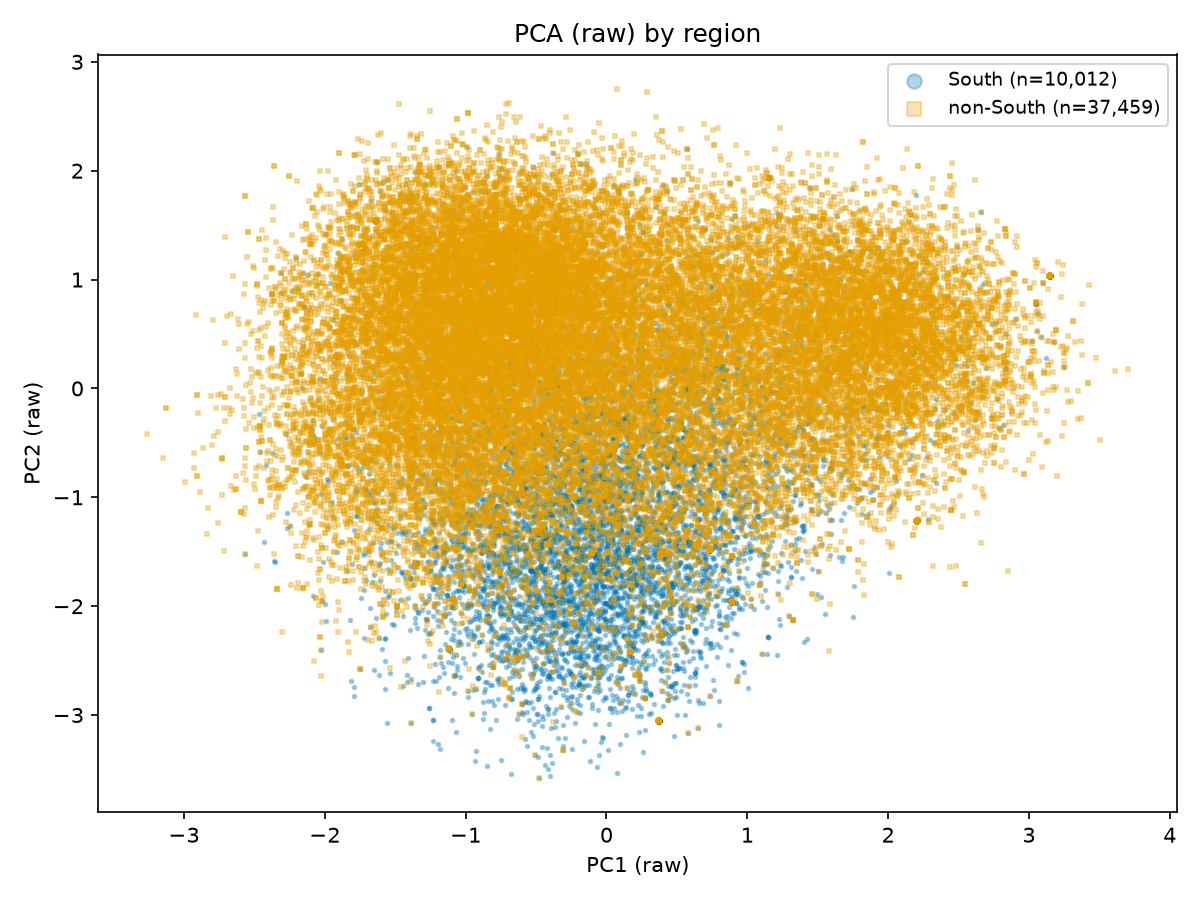
\includegraphics[width=0.32\textwidth]{../figs/pca_raw_region.png}
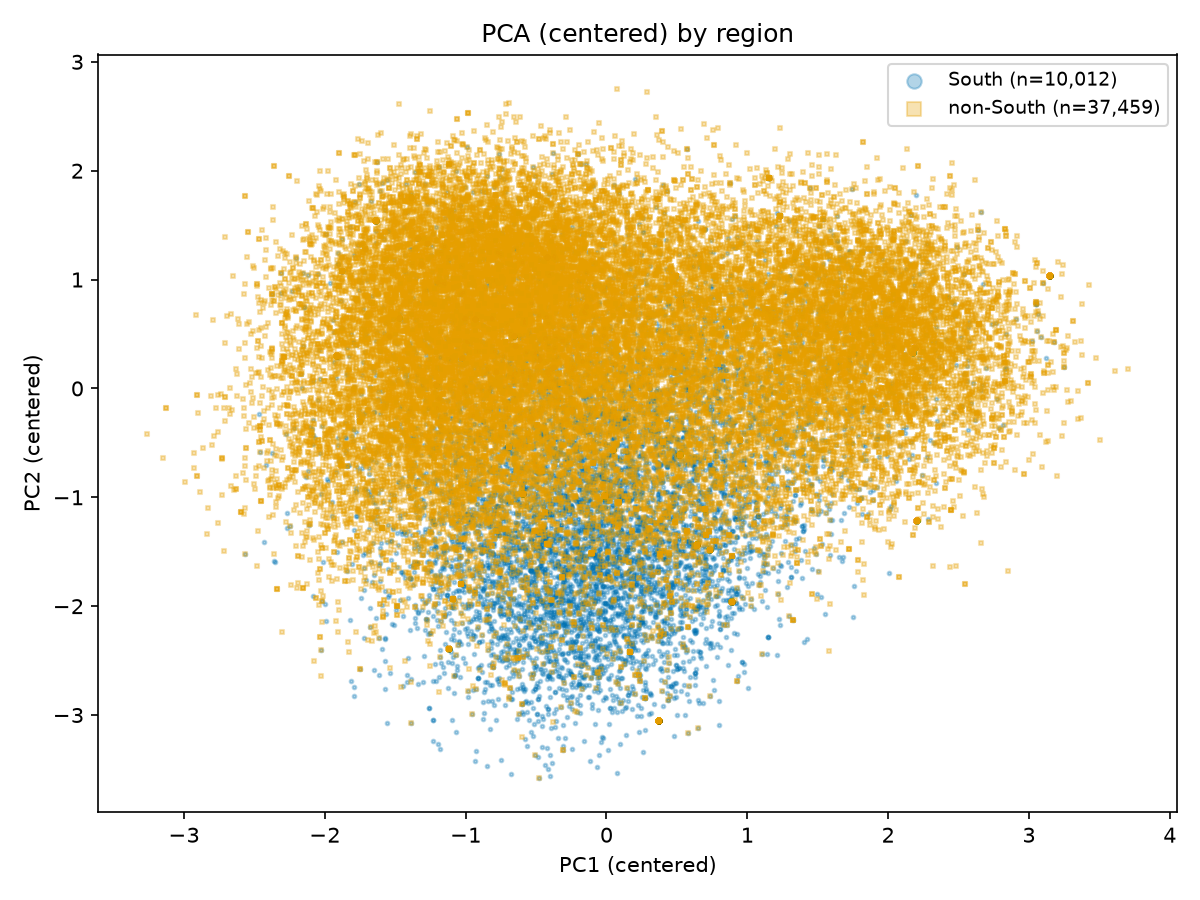
\includegraphics[width=0.32\textwidth]{../figs/pca_centered_region.png}
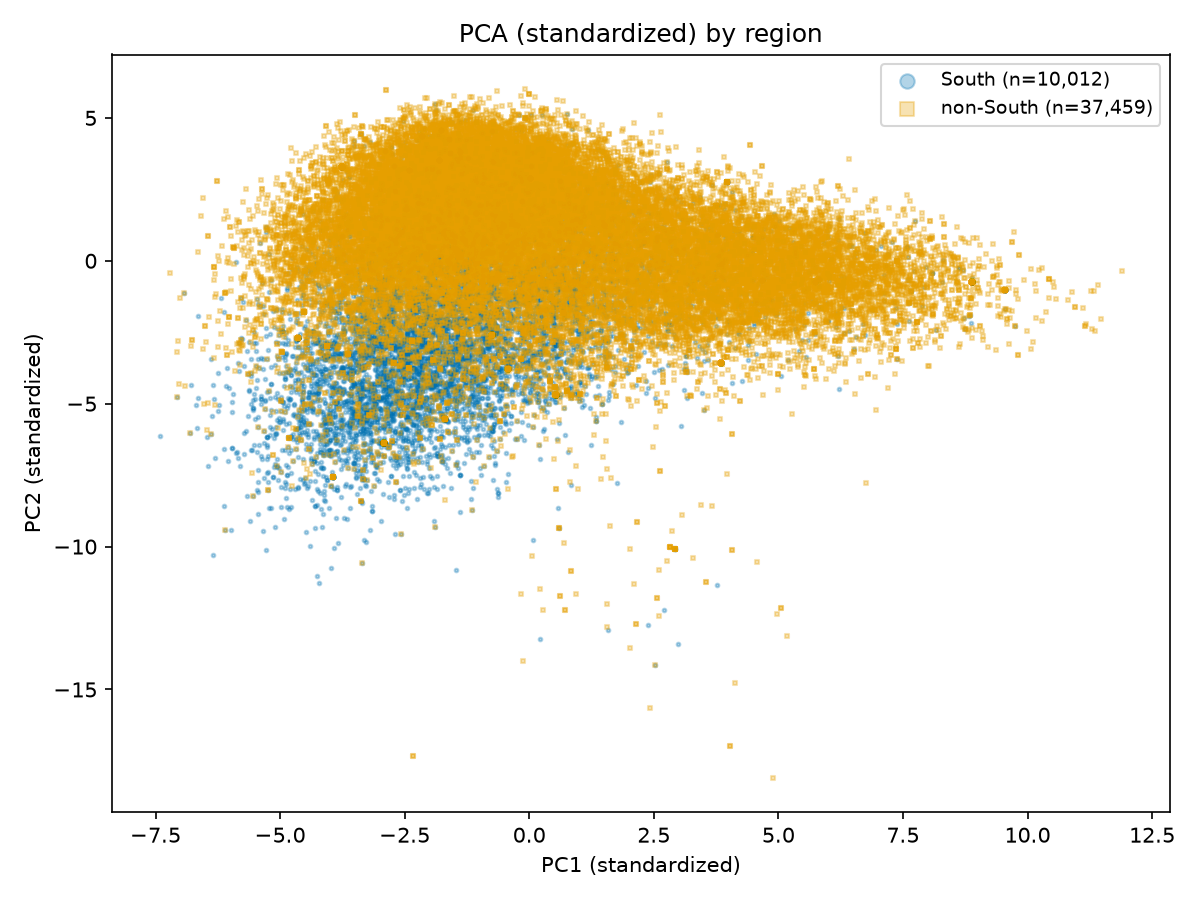
\includegraphics[width=0.32\textwidth]{../figs/pca_standardized_region.png}
\caption{PCA projections of the same respondents, colored by region:
uncentered, centered, and standardized. The first two are identical;
standardization redistributes the coastal group.}
\label{fig:pcacomp}
\end{figure}

Running PCA directly on \texttt{lingData} instead of the encoded matrix would
be actively misleading. The raw codes are labels, not measurements: the gap
between code 4 (\emph{you guys}) and code 9 (\emph{y'all}) is 5, while the gap
between code 4 and code 7 (\emph{you}) is 3, yet these three words are equally
different ways of addressing a group. Euclidean distance in code space would
therefore report that \emph{you-guys} is "closer to" \emph{you} than to
\emph{y'all}, and PCA's variance-maximizing directions would be built on
meaningless arithmetic. One-hot encoding removes the ordering that was never
there.

\subsection{NMF and t-SNE}

PCA assumes linearity and roughly Gaussian variation, which fits count data
poorly. NMF suits binary indicators better because it is constrained to
nonnegative, additive parts. With ten components the parts read as dialect
profiles rather than abstract axes (Figure~\ref{fig:nmf}): one bundles
\emph{sneakers} with \emph{soda} (coastal/urban), another
\emph{tennis shoes} with \emph{crawdad} and \emph{lightning bug} (Southern),
another double-\emph{no} grammar answers with plain \emph{you}
(Northern/Midland). That these cohere into recognizable bundles is the
clearest evidence in the analysis that the regional signal is real and not an
artifact of any one question.

\begin{figure}[h]
\centering
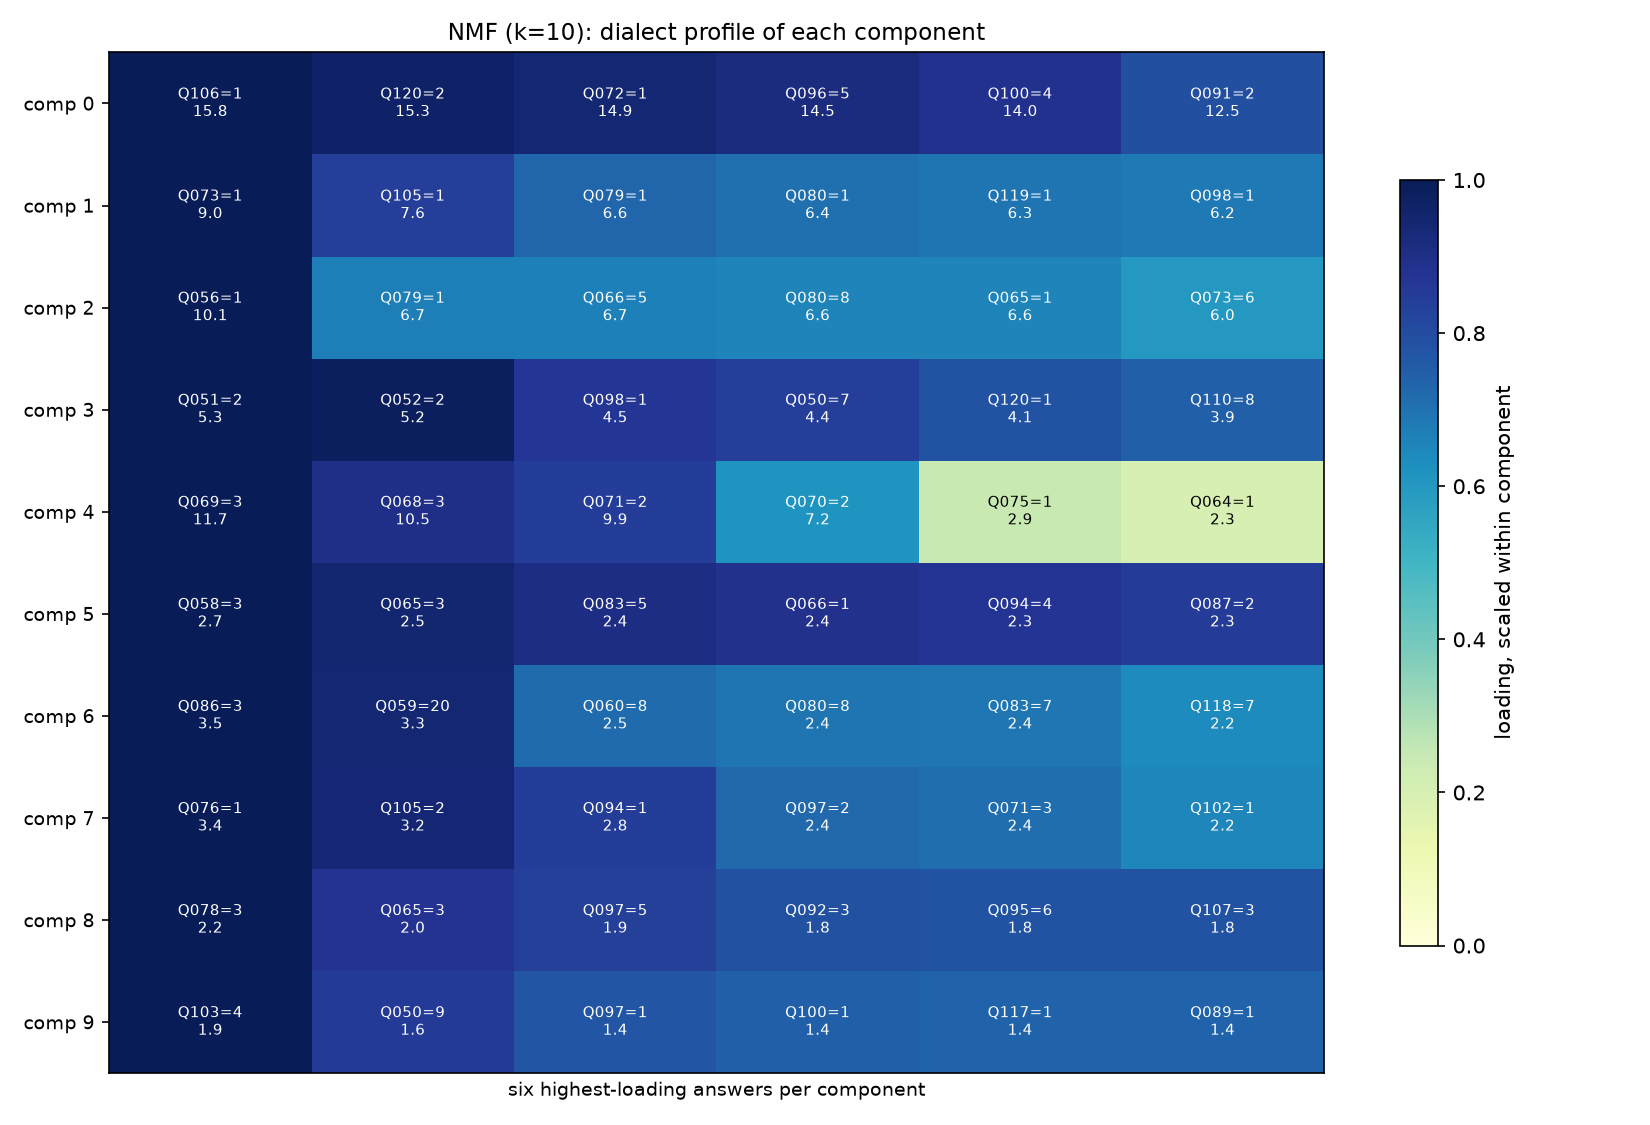
\includegraphics[width=0.82\textwidth]{../figs/nmf_loadings.png}
\caption{NMF with ten components, each showing its six highest-loading
answers. Colour is scaled within a component, since components differ in total
loading by almost a factor of ten. Several read as coherent regional bundles:
component 1 is \emph{sneakers} with \emph{soda}, component 2 pairs
\emph{tennis shoes} with \emph{crawdad} and \emph{lightning bug}, and
component 4 is the kinship set Q068--Q071.}
\label{fig:nmf}
\end{figure}

t-SNE on PCA-50 scores (Figure~\ref{fig:tsne}) gives the sharpest visual
separation: a distinct Southern cloud with the northern respondents forming a
connected mass behind it, and very few points suspended between. Perplexity is
the one parameter worth setting deliberately: it trades local detail against
global structure. I used 50, which preserves the Northern/Midland
sub-structure visible in PCA. I did not sweep it, so a larger value might
separate the regions more cleanly or merge them further, and I cannot say
which.

\begin{figure}[h]
\centering
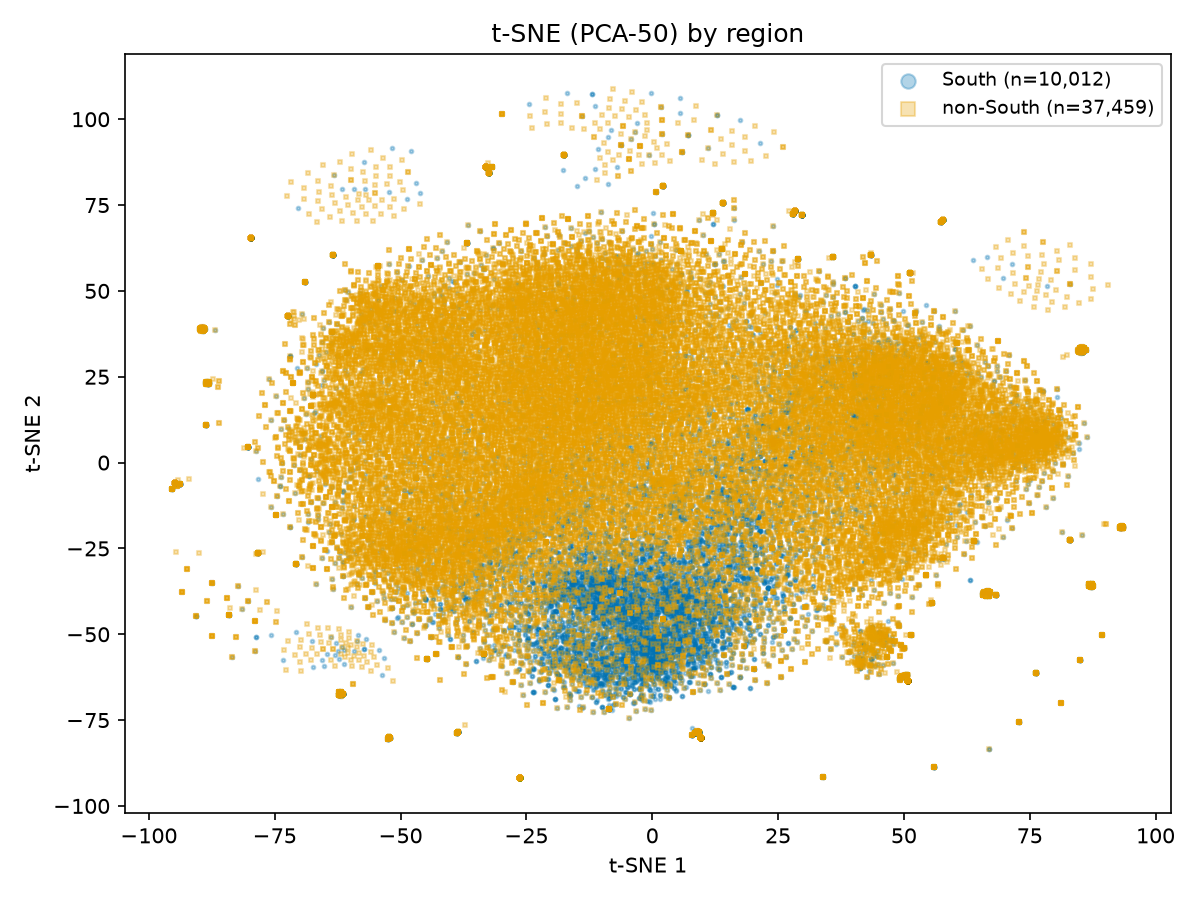
\includegraphics[width=0.56\textwidth]{../figs/tsne_region.png}
\caption{t-SNE on PCA-50 scores (perplexity 50): a distinct Southern cloud with
the northern mass connected behind it.}
\label{fig:tsne}
\end{figure}

\section{Clustering}\label{clustering}

\subsection{Choosing the number of clusters}

Rather than picking $k$ for interpretability first, I swept it. Inertia falls
smoothly with no elbow (1,657,134 at $k=2$ down to 1,524,474 at $k=8$), and
silhouette scores computed on an 8,000-respondent subsample are remarkably
flat: 0.033 at $k=3$, 0.032 at $k=2$ and $k=5$, 0.031 at $k=4$, falling to
0.029 by $k=6$. These are very low values in absolute terms: under
conventional thresholds, the data contain no well-separated groups at any $k$.
What $k=3$ does have is the highest silhouette of the sweep, and the cluster
profiles are interpretable enough to corroborate the choice on their own.

\subsection{k-means on respondents}

Running k-means on the full respondent matrix produces clusters whose modal
answers are immediately interpretable. Sizes are 13,631 / 13,531 / 20,309, and
each cluster has answers that are over-represented within it
(Figure~\ref{fig:profiles}). Cluster 0 is \emph{sneakers} (88.9\% against 37.2\%
overall) and \emph{soda} (84.4\% vs 46.4\%). Cluster 1 is \emph{y'all} (47.3\% vs
17.1\%) and \emph{coke} (37.1\% vs 13.8\%). Cluster 2 is \emph{tp'ing} (82.6\%
vs 58.1\%), \emph{kitty-corner} (71.4\% vs 45.9\%), and \emph{pop} (51.1\% vs
27.5\%).
Mapping them (Figure~\ref{fig:km3}) and cross-tabulating against the four
regions (Table~\ref{tab:clusterregion}) gives Coastal/Northeast, South, and a
third group that is \emph{pop}-leaning but geographically split between the
Midwest and the West, at 65.0\% and 73.9\% of those two regions.

\begin{table}[h]
\centering
\begin{tabular}{lrrr}
\hline
Region & Cluster 0 & Cluster 1 & Cluster 2 \\
\hline
Northeast & 73.2 & 13.8 & 13.0 \\
South & 20.4 & 62.5 & 17.0 \\
Midwest & 10.9 & 24.1 & 65.0 \\
West & 13.3 & 12.7 & 73.9 \\
\hline
\end{tabular}
\caption{Cluster membership by region (row percentages). Cluster 0 =
Coastal/Northeast, cluster 1 = South, cluster 2 = \emph{pop}-leaning interior
and Pacific. Cram\'er's V = 0.512 (n = 47,312).}
\label{tab:clusterregion}
\end{table}

\begin{figure}[h]
\centering
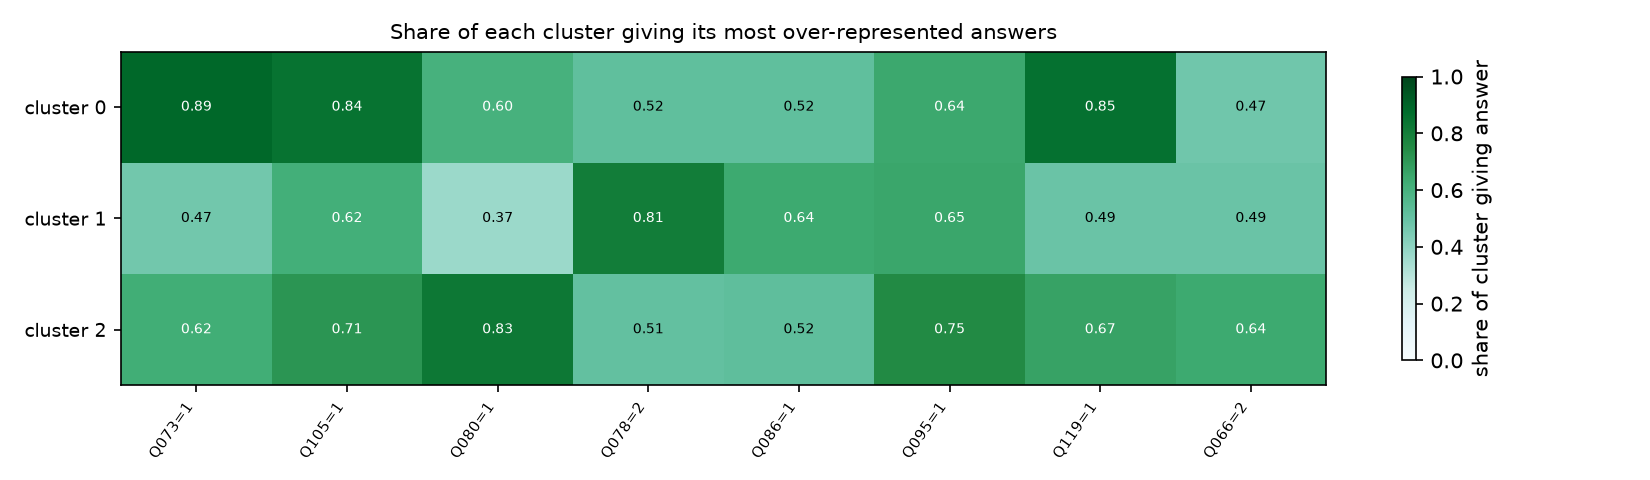
\includegraphics[width=0.82\textwidth]{../figs/cluster_profiles.png}
\caption{The eight answers most over-represented in each k-means cluster, as a
share of that cluster.}
\label{fig:profiles}
\end{figure}

\begin{figure}[h]
\centering
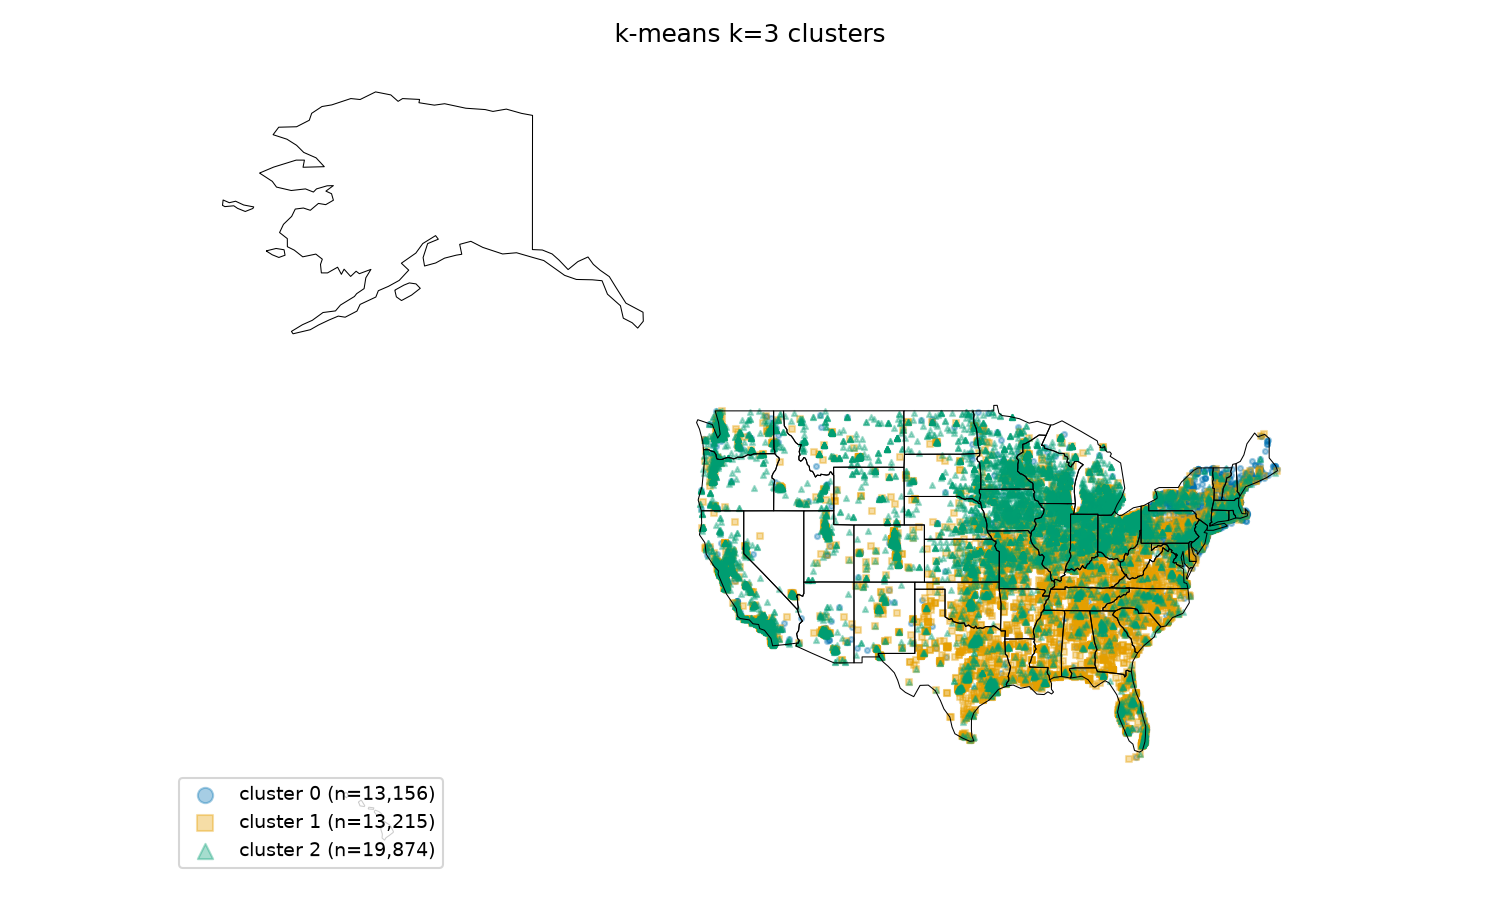
\includegraphics[width=0.74\textwidth]{../figs/kmeans_k3_map.png}
\caption{k-means ($k=3$) clusters mapped: a Northeast/coastal cluster, a Southern
cluster, and a \emph{pop}-leaning interior and Pacific cluster.}
\label{fig:km3}
\end{figure}

The $k=4$ solution is instructive rather than useful: it splits off a cluster
of 1,395 respondents whose modal answers are 0 on both focal questions:
non-responders. Because my encoding maps no-response to zeros, a
missingness pattern becomes a geometrically coherent group, which is exactly
the failure mode one should worry about. Rejecting $k=4$ on these grounds
independently of the silhouette argument is reassuring rather than convenient.

\subsection{Continuum or clusters, and from where to where?}\label{continuum}

The clusters overlap (silhouette $\approx 0.03$), and the gradient figure shows
why: the Southern cluster is not a discrete blob but the high end of a
north--south gradient. Binning respondents into 4-degree latitude bands (finer bins in
Figure~\ref{fig:grad}), P(\emph{y'all}) runs 29\%, 54\%, 36\%, 18\%, 8\%, 7\%
from the Gulf Coast north to the Canadian border, and P(\emph{coke}) tracks it
at 43\% in the Deep South band against 4\% in the north. Longitude tells a
complementary story. In 10-degree bands, P(\emph{y'all}) peaks at 34\% in the
$-105$ to $-95$ band (Missouri, Arkansas, eastern Texas), against 8\% on the
Pacific coast and 9\% in the Mountain West. It rises again to 21\% in the $-85$ to $-75$ band, which
reflects Appalachian and Piedmont populations. So the
continuum runs from the Pacific Coast and Mountain West (soda, \emph{you
guys}), through the Midwest (\emph{pop}), across the Mississippi Valley, to
the Deep South and Appalachia (\emph{coke}, \emph{y'all}), with sharp
enclaves superimposed rather than replacing it.

\begin{figure}[h]
\centering
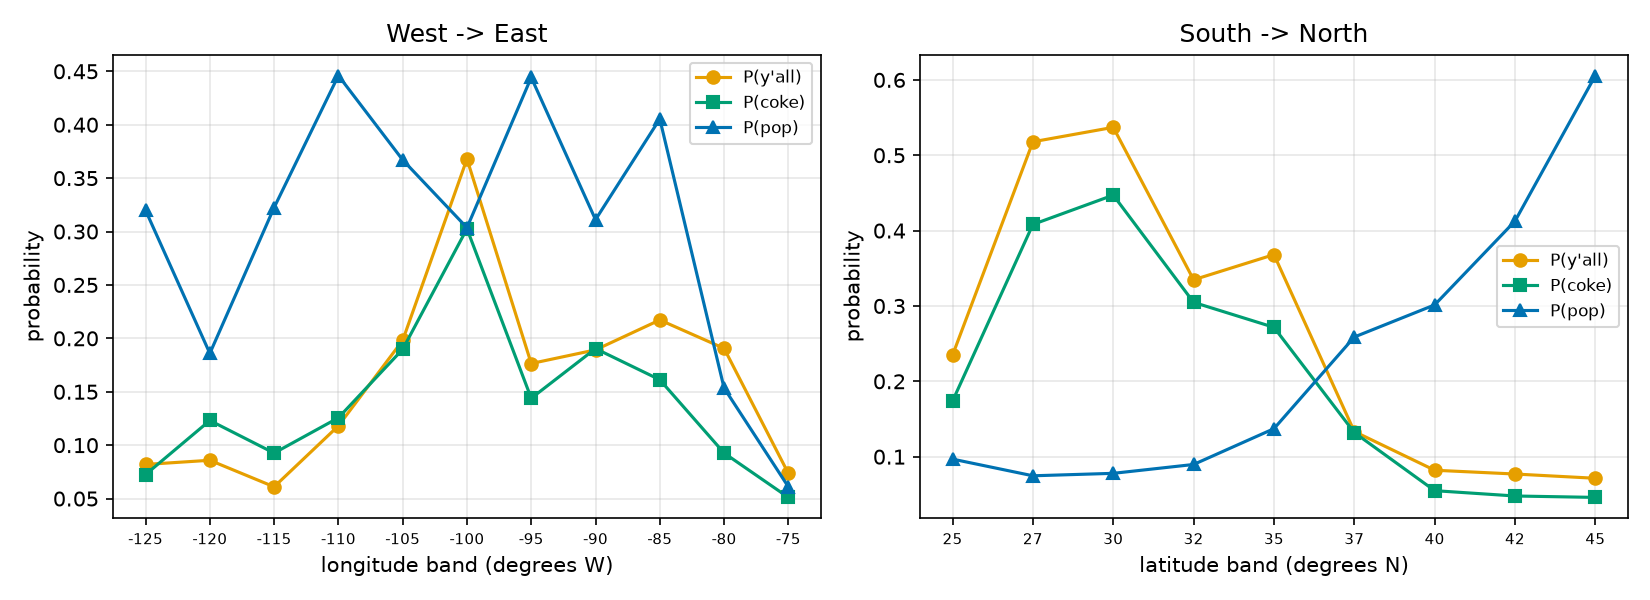
\includegraphics[width=0.78\textwidth]{../figs/continuum_gradient.png}
\caption{P(\emph{y'all}) and P(\emph{coke}) by longitude (left) and latitude
(right): the southern cluster is the high end of a gradient, not an island.}
\label{fig:grad}
\end{figure}

\subsection{Which questions produce the structure?}\label{separators}

Ranking every question by Cram\'er's V against the $k=3$ labels identifies
what drives the partition: Q105 (0.498), Q073 (0.490), Q106 (0.431), Q050
(0.418), Q103 (0.398), Q076 (0.388), Q080 (0.365), Q099 (0.343). At the
bottom, Q057 (0.040) and Q121 (0.066) are essentially uninformative about
region. Table~\ref{tab:separators} lists the extremes. The broad north--south
variables sit at the top (Q105, Q073, Q050), and Q106 (\emph{tp'ing} vs
\emph{toilet papering}) ranks third, which is a reminder that the strongest
separators are not automatically the most interesting dialect variables:
\emph{tp'ing} is a broad informal-register marker that happens to split the
country nearly the way \emph{y'all} does. The genuinely weak separators are
questions whose answers are near-universal nationwide, so they cannot
distinguish anything.

\begin{table}[h]
\centering
\begin{tabular}{lrlrlr}
\hline
\multicolumn{3}{c}{Strongest separators} & \multicolumn{3}{c}{Weakest separators} \\
\hline
Q105 beverage word & 0.498 & & Q115 academic point & 0.080 & \\
Q73 gym shoes & 0.490 & & Q121 ogling & 0.066 & \\
Q106 \emph{tp'ing} & 0.431 & & Q057 \emph{anymore} & 0.040 & \\
Q50 group address & 0.418 & & & & \\
Q103 water fountain & 0.398 & & & & \\
\hline
\end{tabular}
\caption{Cram\'er's V between each question and the $k=3$ cluster labels,
highest and lowest.}
\label{tab:separators}
\end{table}

\subsection{Hierarchical clustering on binned cells}

As a second method I cluster the 781 binned cells of
\texttt{lingLocation.txt}, which directly tests whether geography-based
aggregation changes the picture. The linkage choice dominates the result.
Ward on row-normalized compositions isolates a single 1-person cell as its own
cluster (sizes 318 / 1 / 462 across all 781 cells), because Ward merges on
Euclidean distance and that lone cell sits far from everything. Average linkage
collapses even harder (779 / 1 / 1). Only complete linkage on the 449 cells
with at least 10 respondents gives usable groups (247 / 154 / 48), and it
agrees geographically with k-means' South-versus-rest split.

That agreement does not survive a change of metric. Jaccard distance, the
natural similarity for binary indicator vectors because the thousands of
questions both cells left blank cancel out, puts 444 of the 449 cells in a
single group and agrees with the Euclidean partition at ARI = 0.001. The reason
is visible in the distances themselves: every cell answered 285 of the 468
questions on average, so any two cells agree on most of what they answered and
the pairwise Jaccard distances are small and nearly uniform (median 0.326,
standard deviation 0.082, range 0.054--0.630). With so little to separate on,
average linkage collapses.

The deeper problem is that \texttt{lingLocation.txt} rows are unnormalized
counts, so a cell with many respondents shares indicators with every other
large cell regardless of what was said. Jaccard on this representation partly
measures survey effort rather than speech. The cell-level result is therefore
fragile and metric-dependent, and I would not defend it; the respondent-level
k-means result is the one that holds up.

\subsection{Do the models' assumptions fit the data?}

This is the question the instructions pose about dimension reduction, and the
answer differs by method. PCA's model (orthogonal axes of maximum variance, implied by a
linear-Gaussian picture) fits the \emph{aggregate} structure
well enough to expose the regional gradient, but its flat spectrum and
Gaussian assumption are poor descriptions of 468 sparse indicators; NMF's
nonnegative, additive parts describe them better and yield the most
interpretable components. For clustering, k-means assumes compact spherical
clusters under Euclidean distance, and the silhouette of $\approx 0.03$ says
that assumption is violated: these clusters are not spheres, they are
overlapping regional densities. Complete-linkage agglomerative clustering makes
no distributional assumption at all, which is why it is the more defensible of
the two here, but it assumes every point is worth as much as every other, which
is how the 1-person cell ended up isolated. Neither method's assumptions match
the data perfectly; that both nonetheless recover the same geography is
evidence the signal is robust rather than an artifact of one algorithm. The
practical advantages divide cleanly. k-means scales to 47,471 rows in
seconds and needs only $k$, but it requires a guess at $k$ and can fall into
poor local optima (Section~\ref{stability}). Complete linkage makes no shape
assumption and gives a dendrogram showing structure at every level, and it
is deterministic, but it costs $O(n^2)$ memory and was infeasible at full
respondent count.

\begin{figure}[h]
\centering
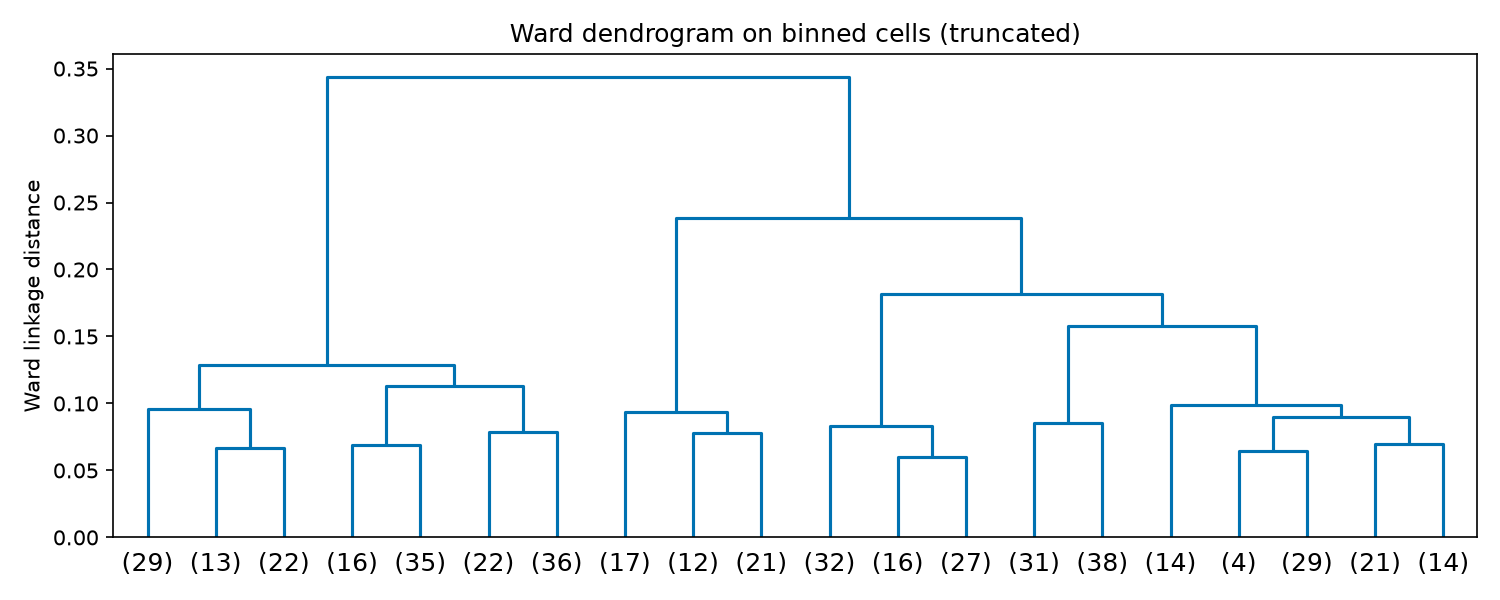
\includegraphics[width=0.36\textwidth]{../figs/agglo_dendro.png}
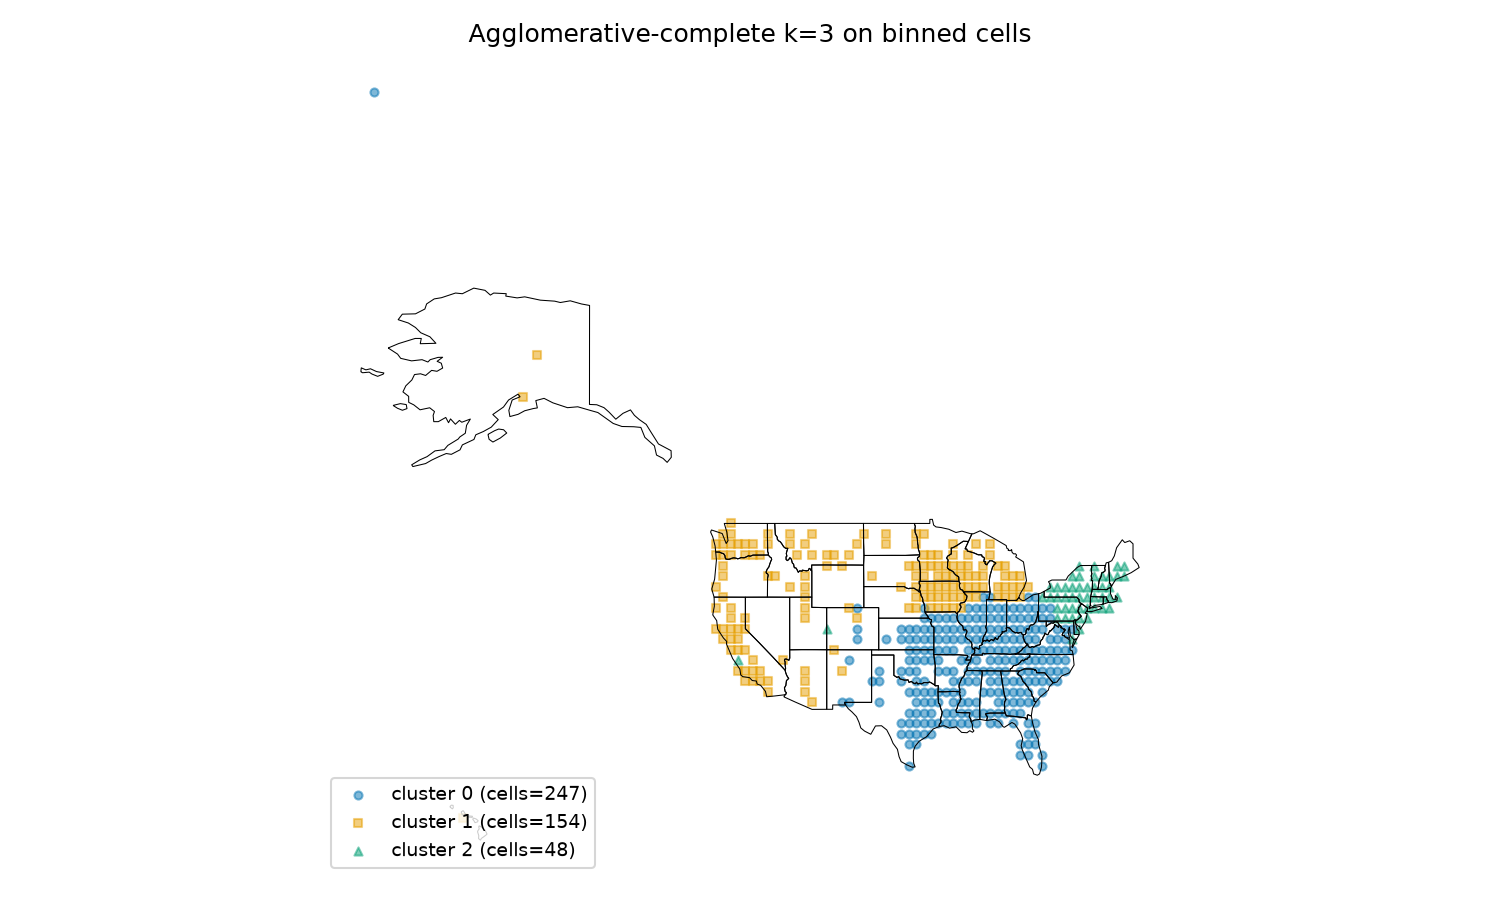
\includegraphics[width=0.62\textwidth]{../figs/agglo_complete_k3_map.png}
\caption{Ward dendrogram on the same 449 adequately populated cells used for
the complete-linkage fit (left), and those complete-linkage clusters ($k=3$,
right). The degenerate Ward solution discussed in the text is computed on all
781 cells.}
\label{fig:agglo}
\end{figure}

\section{Stability of findings to perturbation}\label{stability}

Stability is what separates a regional pattern from an artifact of one run.
Comparing each refit against the full-data $k=3$ partition by Adjusted Rand
Index:

\begin{itemize}
\item \textbf{Different starting points.} Across 10 seeds, mean ARI = 0.944
(minimum 0.803). One seed in ten finds a visibly worse local optimum, which is
the concrete argument for always reporting $n_{\mathrm{init}} \geq 10$ rather
than a single fit.
\item \textbf{Subsampling.} Refitting on ten random 80\% subsamples gives ARI
$0.972 \pm 0.019$ and NMI $0.951 \pm 0.028$, so the partition is essentially
unchanged when a fifth of the respondents are removed, and the modest standard
deviation tracks the southern cluster's boundary, which is where respondents
sit closest to the cluster edges.
\end{itemize}

A third check asks whether the \emph{projection} generalizes, not just the
partition. Fitting PCA on 70\% of respondents, projecting the held-out 30\% onto
those components, then refitting on the held-out data alone, gives $R^2$ =
0.998, 0.997 and 0.998 on the first three components and 0.971 across ten, with
matching-component cosines of 0.92--0.998. PC1 on the unseen respondents still
separates the South (+0.054) from the non-South (-0.023), so the regional axis
is a property of the variables rather than of the rows used to find it.

(Bootstrapping with replacement is the obvious third check, but duplicate row
indices make a point-wise partition comparison ill-defined, so subsampling is
the cleaner stability read here.) The conclusion is that the Southern cluster
is not an artifact of particular rows or a lucky initialization: it survives
both perturbation types with ARI above 0.94, and the geographic gradient in
Figure~\ref{fig:grad}, a smooth monotonic band rather than a fitted
boundary, is the substantive reason to trust it.

\section{Conclusion}\label{conclusion}

\subsection{Three realms}

\textbf{Data.} This survey describes broad regional structure well: the
north--south gradient, the Q50/Q105 interaction, and the local enclaves are all
large, consistent, and visible without modeling. But it is a self-selected web
sample (young, online, English-literate, and not drawn from any probability
frame) with self-reported locations and ZIP-centroid geocoding, so it
supports description, not inference about individuals or small areas.

\textbf{Algorithms.} The clusters are stable (ARI $> 0.94$) but barely
separated (silhouette $\approx 0.03$). That combination says something precise:
the algorithms have found the \emph{density modes} of a continuum, not discrete
populations. Reading cluster boundaries as dialect borders would misread the result:
respondents form overlapping regional dialects, and the three-cluster solution
is a convenient description of three places where those dialects are densest.

\textbf{Future data.} For decisions about people or places, this sample is not
adequate without a probability-based design and survey weighting, and the
geocoding precision is a hard floor on sub-county claims. What the analysis
does support is that region predicts a bundle of lexical choices strongly
enough to be useful for coarse planning where it already holds (language
model training data, speech-recognition dialect coverage, or targeting), and
the Q105 holdout result raises confidence in the southern cluster specifically.

\subsection{Reality check}

The clusters deserve an external test rather than internal consistency, so I
removed the beverage question from the analysis entirely and re-clustered on
the remaining 458 columns. If the southern cluster is a real regional
phenomenon, then respondents who actually said \emph{coke} should land in the
\emph{y'all}-heavy cluster at a much higher rate than chance, without the
beverage question having contributed to that cluster's existence. They do:
the \emph{y'all}-heavy cluster (45.5\% \emph{y'all} against 4.8\% and 5.4\% in
the other two) captures 72.1\% of the 6,550 \emph{coke} respondents, versus
19\% of \emph{pop} respondents and 17\% of \emph{soda} respondents, a
fourfold enrichment. Part of this signal flows through Q050 itself, since
\emph{y'all} and \emph{coke} are themselves correlated, so the check validates
the cluster's geography more than it replicates the beverage finding
independently. It is still informative: the clustering never had access to
any beverage information.

\subsection{Impact and what I would add next}

The domain-level conclusion is that the large dialect features the literature
describes are all present here (a northern/southern lexical divide, a
Midland \emph{pop} belt, sharp metropolitan enclaves), and that the
aggregate-measurement approach Nerbonne and Kretzschmar advocate does recover
them from noisy individual words. On the survey's own website the words I
clustered on are collected precisely because they are expected to be
geographically diagnostic, and they behave that way.

With more time I would add several things. Aggregating to counties would let me
test whether the enclaves (\emph{hoagie}, \emph{bubbler}) sharpen or dissolve
once the population base is large enough to estimate them reliably, since
clustering the current data necessarily down-weights exactly those rare
answers. Surveying age and year of response would allow the more interesting
question of whether these dialects are stable or undergoing convergence.
Proper survey weighting would let the regional percentages mean what people
think they mean. And a Jaccard-distance hierarchical clustering would give a
similarity measure appropriate to binary indicator vectors, rather than
Euclidean distance on a matrix where every point shares most of its zeros.

\section{Academic honesty statement}\label{academic-honesty-statement}

I personally designed and carried out all data analysis procedures presented in this report. I wrote the report and created the figures myself. I used an LLM in the limited ways permitted by the course policy. For writing, I used it to brainstorm possible ways to improve wording and presentation and to suggest edits to grammar, wording, and sentence flow in text that I had already written. I did not use an LLM to generate paragraphs or produce report content from bullet points.

For coding, I used an LLM to brainstorm possible approaches and for suggestions related to parts of the modeling and sensitivity-check code, as well as figure revisions. I reviewed and understood the suggested code before using or adapting it and remained responsible for the final implementation and analysis.

I believe academic honesty is a fundamental requirement for conducting research. Researchers need to take responsibility for the results they produce because science builds on collaboration and on the work of others. If research is dishonest or cannot be reproduced, it can become the basis for further research and potentially lead to a chain of incorrect conclusions. Academic work should also be original and properly acknowledge the contributions of others. Plagiarism does not contribute new work to the scientific community and fails to give appropriate credit to the original authors. For these reasons, research should be conducted in an honest and reproducible way.

\section{Collaborators}\label{collaborators}

None.


\section*{Bibliography}
\begin{itemize}
\item J. Nerbonne and W. Kretzschmar, Jr., ``Introducing computational
techniques in dialectometry,'' \textit{Computers and the Humanities}
37:245--255, 2003.
\item J. Nerbonne, ``Progress in dialectometry: toward explanation,''
\textit{Literary and Linguistic Computing}, 2006.
\item B. Vaux, \emph{Dialect Survey}, \url{https://www.dialectsofenglish.com/}.
\end{itemize}

\end{document}